\documentclass{article}
\usepackage{arxiv}
\usepackage{wrapfig}
\usepackage{amsmath}
\usepackage[utf8]{inputenc}
\usepackage[english, russian]{babel}
\usepackage[T1]{fontenc}
\usepackage{url}
\usepackage{booktabs}
\usepackage{float}
\usepackage{amsfonts}
\usepackage{nicefrac}
\usepackage{microtype}
\usepackage{lipsum}
\usepackage{amssymb}
\usepackage{graphicx}
\usepackage{natbib}
\usepackage{doi}

\pagestyle{fancy}



\title{Восстановление прогноза, сделанного в метрическом вероятностном пространстве, в исходное пространство (временных рядов)}

\author{ Maxim Divilkovskiy \\
% \thanks{Use footnote for providing further
% 		information about author (webpage, alternative
% 		address)---\emph{not} for acknowledging funding agencies.} \\
	Chair of Data Analysis\\
	MIPT\\
	\texttt{divilkovskii.mm@phystech.edu} \\
	%% examples of more authors
	\And
	Vadim Strijov \\
	FRC CSC of the RAS\\
	Moscow, Russia\\
    \texttt{strijov@phystech.edu} \\
    \And
    Yakovlev Konstantin \\
    Chair of Intellectual Systems\\
    MIPT\\
    \texttt{iakovlev.kd@phystech.edu} \\
	% Santa Narimana, Levand \\
	% \texttt{stariate@ee.mount-sheikh.edu} \\
	%% \AND
	%% Coauthor \\
	%% Affiliation \\
	%% Address \\
	%% \texttt{email} \\
	%% \And
	%% Coauthor \\
	%% Affiliation \\
	%% Address \\
	%% \texttt{email} \\
	%% \And
	%% Coauthor \\
	%% Affiliation \\
	%% Address \\
	%% \texttt{email} \\
}
\date{}

\renewcommand{\shorttitle}{\textit{arXiv} Template}

%%% Add PDF metadata to help others organize their library
%%% Once the PDF is generated, you can check the metadata with
%%% $ pdfinfo template.pdf
\hypersetup{
pdfauthor={Maxim Divilkovskiy},
}

\graphicspath{ {./figures/} }

\begin{document}
\maketitle

\begin{abstract}
	Решается задача поточечного прогнозирования набора временных рядов с высокой ковариацией и высокой дисперсией. Для решения данной задачи предлагается построить пространство парных расстояний. В этом пространстве прогнозируется матрица попарных расстояний, а затем по известной матрице восстанавливаются значения временных рядов.
	В данной статье изучается способ восстановления прогноза в пространстве временных рядов по известной матрице попарных расстояний. Показывается недостаточность одной матрицы попарных расстояний. Предлагается несколько алгоритмов, основанных на использовании нескольких матриц, построенных по различным временным интервалам с использованием попарной корреляции. Так же, в статье выводится общий вид восстановленных значений. Помимо этого, приводится оценка качества восстановления при добавлении шума в матрицы попарных расстояний.


\end{abstract}


\keywords{Metric \and Trades \and Correlation \and Time Series Forecasting}

\section{Введение}
	Цель данной работы заключается в представлении нового метода поточечного прогнозирования временных рядов, характеризующихся высокой попарной ковариацией и высокой дисперсией. Задача заключается в прогнозировании значений временных рядов в следующий момент по имеющимся историческим данным. Задача разбивается на три этапа: сначала исходное пространство временных рядов трансформируется в метрическое пространство при помощи построения матрицы попарных расстояний, затем в этом пространстве осуществляется прогноз матрицы попарных расстояний в следующий момент времени. В теоретической части статьи показана необходимость прогноза не менее чем двух матриц, отвечающих различным подотрезкам времени, для единственности ответа. Последним этапом, по спрогнозированным данным результат возвращается в исходное пространство. Статья фокусируется в первую очередь на последнем этапе. Приводятся эксперименты в случае с точным прогнозом матрицы с добавлением к значениям нормального шума.
		
	Существующие способы предсказания временных рядов, такие как LSTM \cite{LSTM}, SSA \cite{SSA} и другие \cite{Biosignals}, \cite{boyd2017multiperiod} основаны на предсказании значения одного ряда. При этом, данные методы могут быть изменены для прогноза в том числе набора временных рядов, если рассматривать набор рядов как один многомерный ряд. Однако, такой подход не моделирует в явном виде зависимости между различными рядами. В данной работе предлагается анализировать изменение набора временных рядов, явно используя связи между ними в качестве информации. Подобное исследование проводится в статье \cite{MulticorrelatedQuadratic}, однако в ней делается упор на задаче feature selection. Данная задача заключается в выборе такого поднабора из исходных временных рядов, для которых возможно делать прогноз достаточного качества.
	
	Новизна работы заключается в том, что прогнозирование делается не в исходном пространстве, а в пространстве попарных расстояний, способ построения которого предложен в статье. Преимущество данного метода заключается в том, что в реальных наборах временных рядов (природных, физических, финансовых и т.д.), часто наблюдается зависимость, близкая к линейной. Эта дополнительная информация способна улучшить качество итогового прогноза. Помимо этого, прогнозируемую матрицу можно рассматривать как набор временных рядов. В этом случае размерность данных возрастает до $O(n^2)$ против $n$ рядов, что увеличивает информативность входных данных.
	
	Далее рассматриваюся условия на функцию расстояния между рядами при которых существует способ восстановления значений временных рядов. Доказывается недостаточность одной матрицы для восстановления ответа. Предлагается два метода, использующие несколько матриц, для случая точного прогноза и для случая прогноза с погрешностью. Так же предлагается алгоритм восстановления, основанный на двух теоремах о явном виде ответа при использовании попарной корреляции в качестве функции попарного расстояния между рядами.

\section{Постановка задачи}

Ниже приведена постановка задачи поточечного прогнозирования набора временных рядов в общем виде.

Набор из $d$ временных рядов задан $t$ векторами:

$$[\mathbf{x}_1, \mathbf{x}_2, \ldots, \mathbf{x}_t], \text{для всех } k: \mathbf{x}_k \in \mathbb{R}^d, $$

$\mathbf{x}_{t_i, k}$ задаёт собой значение ряда с индексом $k$ в момент времени $t_i$.

Задача заключается в прогнозе $\mathbf{x}_{t+1}$.

$\mathbf{x}$ рассматривается как \textit{многомерный} временной ряд, рассматривая значение в точке как элемент пространства $\mathbb{R}^d$.

В качестве критериев качества используются MSE и MAE. В статье \cite{jadon2022comprehensive} показано, что они являются наиболее подходящими для задачи прогнозирования временных рядов.

\textbf{Общий вид алгоритма при прогнозе одной матрицы расстояний}

1. Строятся матрицы расстояний по предыдущим шагам. Способ построения описан далее.

\begin{align*}
	[\mathbf{x}_1, \ldots, \mathbf{x}_s] &\rightarrow \Sigma_s \\
	[\mathbf{x}_2, \ldots, \mathbf{x}_{s+1}] &\rightarrow \Sigma_{s+1} \\
	&\vdots \\
	[\mathbf{x}_{t-s}, \ldots, \mathbf{x}_t] &\rightarrow \Sigma_{t}
\end{align*}

2. По этим матрицам прогнозируется матрица $\hat{\Sigma}_{t+1}$

3. Найти такой $\hat{x}_{t+1}$, что \[ ||\hat{\Sigma}_{t+1} - \bar{\Sigma}_{t+1}||_2^2 \] минимальна, где $\bar{\Sigma}_{t+1}$~--- матрица расстояний, построенная по набору $[\vec{x}_{t-s+1}, \ldots, \hat{x}_{t+1}]$. Достижение минимума этой функцией будет означать равенство $\hat{\Sigma}_{t+1}$ и $\bar{\Sigma}_{t+1}$. В свою очередь, это означает что найденное продолжение ряда на момент времени $t+1$ имеет матрицу расстояний, равную прогнозу. В общем случае, данная функция невыпуклая и минимумов может быть несколько.

\section{Недостаточность матрицы попарных расстояний для восстановления ответа}

Остутствие единственности решения задачи минимизации, описанной выше, является центральной проблемой, рассматриваемой в данной статье. В данной секции показывается, что только по матрице, построенной по произвольной метрике, невозможно однозначно восстановить значение рядов в следующий момент времени.

Ниже рассматривается возвращение прогноза из матрицы $\Sigma_{t+1}$ в пространство временных рядов, где $\Sigma_{t+1}$ есть матрица попарных расстояний, отвечающая многомерному ряду $\mathbf{x}=[\mathbf{x_1}, \ldots, \mathbf{x_{t+1}}]$.

Пусть дана предсказанная матрица попарных расстояний $\Sigma$ размера $d \times d$ для многомерного временного ряда $\overline{X} \in \mathbb{R}^{d \times (t+1)}$. Предсказывается $y \in \mathbb{R}^d$. Так же, известна метрика $d : \mathbb{R}^{t+1} \times \mathbb{R}^{t+1} \rightarrow \mathbb{R}$, введённая на временных рядах, обладающая свойствами метрики. То есть, $\Sigma_{i,j} = d(X_i \circ y_i, X_j \circ y_j)$, где $\circ$ означает конкатенацию векторов.

В качестве примера рассмотрим евклидову метрику: 

$$d(X_i \circ y_i, X_j \circ y_j)=\sqrt{\left(\sum_{k=1}^t (X_{ik}-X_{jk})^2\right) + (y_i-y_j)^2}.$$

Использование данной метрики приводит к тому, что прибавление ко всем $y_i$ некоторой константы $C$ не изменяет ответ. В случае задачи предсказывания временных рядов это свойство критично, поскольку даже в случае точного предсказания матрицы $\Sigma$ существует бесконечно много значений временных рядов в момент времени $t+1$, отвечающих этой матрице.

\begin{figure}[H]
	\centering
	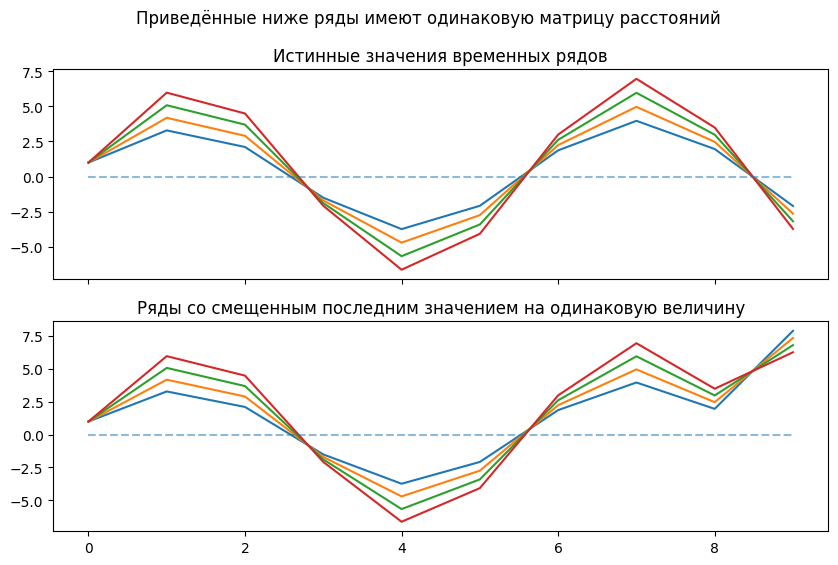
\includegraphics[width=\textwidth]{SameMatrix.png}
	\label{fig:fig1}
\end{figure}

Это приводит к невозможности использования алгоритма MDS для восстановления ответа в исходное пространство временных рядов.

Однако, даже использование других метрик не позволяет избавиться от проблемы.

\textbf{Теорема 1.} \textit{Для любой метрики, введённой в пространстве временных рядов $\mathbb{R}^t$, существует более одного способа восстановить исходные временные ряды из построенной по данной метрике матрице попарных расстояний.}

\textbf{Замечание.} В данном утверждении не используется информация о первых $t-1$ значениях ряда. В сущности, ряд в данном случае можно рассматривать в качестве точки в пространстве $\mathbb{R}^t$. Использование информации о предыдущих моментах времени приведено после данной теоремы.

\textbf{Доказательство.} Достаточно показать, что метрика не является биекцией. Это будет означать, что существуют несколько различных пар рядов, расстояние между которыми одинаковое.

Покажем, что метрика~--- непрерывная функция. Возьмём последовательность \[\{(x_n, y_n)\} \subset \mathbb{R}^t \times \mathbb{R}^t, (x_n, y_n) \to (x, y).\] Тогда, \[x_n\to x, y_n\to y \Rightarrow d(x_n,x)\to 0 ,d(y_n,y)\to 0,\] $при n \to \infty.$ Воспользовавшись неравенством треугольника для метрики, получаем \[d(x_n,y_n)\leqslant d(x_n,x)+d(x,y)+d(y_n,y)\to d(x,y),\] следовательно, $d(x_n,y_n)\to d(x,y)$.

То есть метрика~--- непрерывное отображение из $\mathbb{R}^t \times \mathbb{R}^t$ в $\mathbb{R}$. Покажем, что такое отображение не может быть гомеоморфизмом. Предположим, что $f: \mathbb{R} \to \mathbb{R}^t \times \mathbb{R}^t$~--- искомый гомеоморфизм. Возьмём некоторую точку $a \in \mathbb{R}$ и $f(a)$. Выкинув точку $a$, $\mathbb{R}$ перестаёт быть связным, а $\mathbb{R}^t \times \mathbb{R}^t$ нет. Значит, это не гомеоморфизм. Противоречие.
$\blacksquare$

\textbf{Замечание.} Существенно, в доказательстве используется только непрерывность функции. Это означает, что даже не метрические функции не дадут единственность ответа. Например, попарная корреляция рядов тоже является непрерывной функцией.

Таким образом, зная только матрицу расстояний невозможно однозначно восстановить исходные ряды. В частности, это не позволяет использование алгоритма Multi-Dimensional Scaling. Данный алгоритм часто применяется при восстановлении объектов из информации об их попарном расстоянии.

Рассмотрим ту же задачу, помимо матрицы $\Sigma_{t+1}$ воспользовавшись значением ряда до момента времени $t$: $\mathbf{x}=[\mathbf{x_1}, \ldots, \mathbf{x_{t}}]$. Задача переформулируется следующим образом:

Имеется $n$ объектов в $\mathbb{R}^{t+1}$, известны их первые $t$ координат. Так же известна матрица расстояний $\Sigma_{t+1} \in \mathbb{R}^{(t+1) \times (t+1)}$. Требуется восстановить $t+1$ координату каждого из объектов. В терминах временных рядов, $t+1$-я координата является значением каждого из рядов в этот момент времени.

\section{Попарная корреляция}

В данной секции исследуется восстановление ответа при помощи матрицы попарной корреляции. Такая функция расстояния используется, поскольку в статье \cite{puchkin2023sharper} показано, что оценка попарной корреляции выборки аппроксимирует своё математическое ожидание.

Матрица попарных расстояний строится следующим образом:
\begin{gather*}
	{\Sigma}_T = \frac{1}{T} \sum_{t=1}^{T} (x_t - \mu_T)(x_t - \mu_T)^\mathsf{T},\\
	\mu_T = \frac{1}{T} \sum_{t=1}^{T} x_t.
\end{gather*}

\textbf{Теорема 2.} \textit{В случае, если мы точно спрогнозировали матрицу расстояний, функция} $||\hat{\Sigma}_{t+1} - \bar{\Sigma}_{t+1}||_2^2$ \textit{будет иметь два минимума, задающихся явно следующим образом:}

\begin{align*}
	\hat{y_i} &= y_i,\\
	\hat{y_i} &= \frac{2}{T-1} \sum_{k=1}^{T-1} a_{ik} - y_i,
\end{align*}
\textit{где} $\hat{y}_i$~--- $i$\textit{-я координата предсказываемого значения ряда в момент $T+1$, $A=(a_{ik})$~--- исходный многомерный временной ряд,} $y_i$~--- \textit{истинные значения ряда в момент} $T+1$.

\textbf{Доказательство.} Обозначим за $\Sigma$~--- истинную матрицу в момент времени $T$, а $\hat{\Sigma}$~--- спрогнозированную. По построению, ${\Sigma} = \frac{1}{T} \sum_{k=1}^{T} (a^T_k - \mu_T)(a^T_k - \mu_T)^T$. Матрица $A$ представляет собой транспонированную матрицу $X$ временных рядов, первая размерность~--- номер ряда, а не момент времени как в случае с $X$. Тогда, рассмотрим чему равны элементы матриц $\Sigma$ и $\hat{\Sigma}$.

\begin{align*}
	\Sigma_{ij} &= \frac{1}{T}\sum_{k=1}^{T}(a_{ik} - \mu_i)(a_{jk}-\mu_j),\\
	\hat{\Sigma}_{ij} &= \frac{1}{T}\sum_{k=1}^{T-1}(a_{ik} - \hat{\mu}_i)(a_{jk}-\hat{\mu}_j) + (y_i - \hat{\mu}_i)(y_j - \hat{\mu}_j).
\end{align*}

Поскольку мы минимизируем норму разности, обе матрицы равны друг другу. Рассмотрим равенство диагональных элементов.

\begin{gather*}
	\text{Для любых } i, j \text{ таких, что } i = j \text{ верно: } \Sigma_{ii} = \hat{\Sigma}_{ii},\\
	\sum_{k=1}^{T}(a_{ik} - \mu_i)(a_{ik}-\mu_i) = \sum_{k=1}^{T-1}(a_{ik} - \hat{\mu}_i)(a_{ik}-\hat{\mu}_i) + (y_i - \hat{\mu}_i)(y_i - \hat{\mu}_i),\\
	(a_{iT}-\mu_i)^2 = (y_i-\hat{\mu}_i)^2.\\
	\text{Распишем } \hat{\mu}_i \text{ и } \hat{\mu}:\\
	\hat{\mu}_i = \frac{1}{T}\sum_{k=1}^{T-1}a_{ik} + \frac{1}{T}y_i,\\
	\mu_i = \frac{1}{T}\sum_{k=1}^{T}a_{ik},\\
	\left[
	\begin{array}{ll}
		\frac{T-1}{T}y_i-\frac{1}{T}\sum_{k=1}^{T-1}a_{ik}=a_{iT}-\mu_i
		\\[1ex]
		\frac{T-1}{T}y_i-\frac{1}{T}\sum_{k=1}^{T-1}a_{ik}=\mu_i-a_{iT}
	\end{array},
	\right .\\[1ex]
	\left[
	\begin{array}{ll}
		\frac{T-1}{T}y_i = \frac{T-1}{T}a_{iT}
		\\[1ex]
		\frac{T_1}{T}y_i = \frac{2}{T} \sum_{k=1}^{T-1} a_{ik} - \frac{T-1}{T}a_{iT}
	\end{array},
	\right .\\[1ex]
	\left[
	\begin{array}{ll}
		y_i = a_{iT}
		\\[1ex]
		y_i = \frac{2}{T-1} \sum_{k=1}^{T-1} a_{ik} - a_{iT}
	\end{array}.
	\right .
\end{gather*}

Переобозначив, получаем
\begin{align*}
	\hat{y_i} &= y_i,\\
	\hat{y_i} &= \frac{2}{T-1} \sum_{k=1}^{T-1} a_{ik} - y_i.
\end{align*}
$$ \blacksquare $$

\textbf{Следствие. (Тривиальный метод получения пары возможных ответов.)} Данная теорема показывает что использование попарной корреляции в качестве функции расстояния даёт не более двух различных ответа при восстановлении. Более того, получив один, можно явным образом найти второй. Тогда, для нахождения возможных ответов предлагается применить какой-либо метод невыпуклой оптимизации для нахождения хотя бы одного из минимумов функции.

\begin{figure}[H]
	\centering
	\begin{center}
		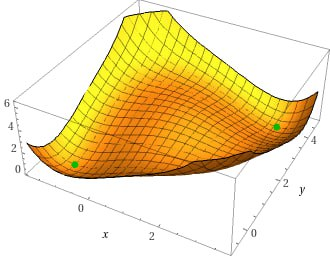
\includegraphics[width=0.5\textwidth]{CorrelationError}
		\label{fig:fig5}
	\end{center}
	\caption{Вид функции $||\hat{\Sigma}_{t+1} - \bar{\Sigma}_{t+1}||_2^2$ для двух рядов: $(1, 3)$ и $(2, 4)$. Точки минимума: (3; 4)~--- искомая и (-1; 0)~--- альтернативная}
\end{figure}


Проблемой данного метода является вычислительная затратность методов невыпуклой оптимизации. В качестве альтернативы предлагается следующий метод, использующий только лишь сингулярное разложение матрицы.

\textbf{Теорема 3. (Быстрый метод получения пары возможных ответов.)} \textit{Минимум функции $||\hat{\Sigma}_{t+1} - \bar{\Sigma}_{t+1}||_2^2$ достигается на \[\pm\sqrt{\lambda_1} u_1 + \mu_t,\] где $\lambda_1$--- первое сингулярное значение, $u_1$--- первый левый сигнулярный вектор матрицы $A=\left(\frac{t}{t+1} \cdot \Sigma_t - \Sigma_{t+1}\right) \cdot \frac{(t+1)^2}{t}$}

$\bigskip$

Эта теорема позволяет находить оба минимума функции намного быстрее, чем при использовании стандартных методов оптимизации.

\subsection{Алгоритм прогноза}

Представленные выше алгоритм возвращает два ответа, из которых невозможно выбрать нужный.

Предлагается следующий алгоритм:

1. Зафиксируем $T$ и $T': T \neq T'$.

2. Для $T$ и $T'$ произведем полученный выше алгоритм и получим наборы ответов: $[ans_1, ans_2], [ans'_1, ans'_2]$.

3. Найдём тот ответ, который лежит в пересечении.


\begin{figure}[H]
	\centering
	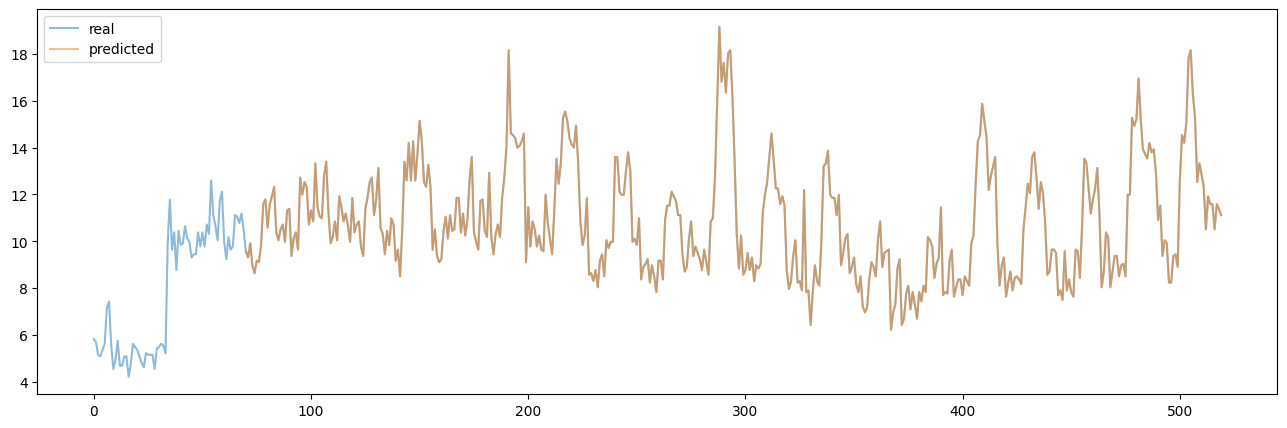
\includegraphics[width=\textwidth]{TwoTAlgo.png}
	\caption{Возвращение прогноза при идеальном прогнозе Sigma. $T=20$, $T'=10$}
	\label{fig:fig3}
\end{figure}

\subsection{Алгоритм при неидеальном прогнозе}

Проблема вышеописанного алгоритма заключается в том, что при неидеальном прогнозе, пересечения может не быть. Более того, если брать два ответа с минимальным расстоянием, мы можем взять не ту пару ответов.

Вместо двух значений  $T$ и $T'$ предлагается брать $K$ значений.

Тогда мы молучим $K$ наборов ответов:

\begin{gather*}
	[ans_{11}, ans_{12}],\\
	[ans_{21}, ans_{22}],\\
	\vdots \\
	[ans_{K1}, ans_{K2}]
\end{gather*}

Далее предлагается перебрать $2^K$ наборов ответов и выбрать тот набор, в котором диаметр минимален.

Асимптотическая сложность данного восстановления будет $O(2^K \times K \times N)$ + сложность используемого алгоритма поиска минимума.

\begin{figure}[H]
	\centering
	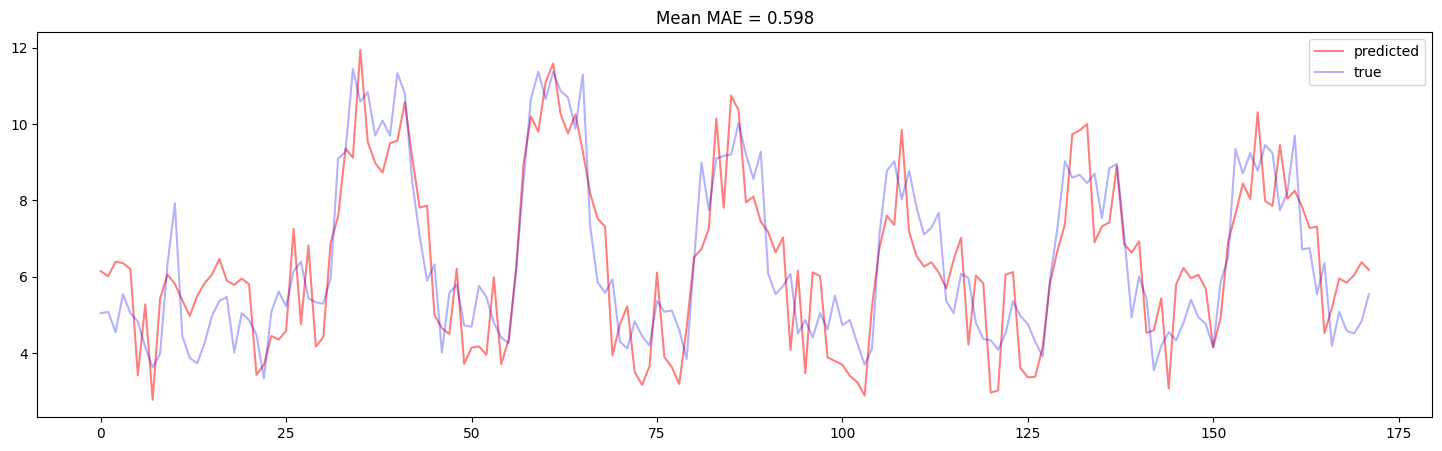
\includegraphics[width=\textwidth]{TbiLSTM.png}
	\caption{Возвращение прогноза при неидеальном прогнозе Sigma при помощи Bidirectional LSTM}
	\label{fig:fig4}
\end{figure}

\section{Computational Experiment}

Исследуются следующие алгоритмы прогнозирования:

\begin{itemize}
	\item LSTM \cite{LSTM}
	\item SARIMA \cite{ARIMAvsLSTM}
	\item LSTM на матрице расстояний
	\item Bidirectional LSTM на матрице расстояний
\end{itemize}

\subsection{LSTM}

LSTM, в отличии от обыкновенной RNN позволяет выделять как кратковременные, так и долговременные зависимости, что позволяет с довольно высокой точностью прогнозировать временные ряды.

В качестве теста используется зашумленный временной ряд длины T, состоящий из суммы синусов и косинусов разных амплитуд и сдвигов. Из этого временного ряда генерируется выборка следующим алгоритмом:\\
1. Выбирается размер окна $W$.\\
2. Ряд разбивается на $T-W-1$ окон размера $W+1$ со сдвигом 1. Эти окна будут семплами\\
3. В каждом из полученных окон первые $W$ будут аргументами на данном семпле, а последнее~--- результатом.

Ряд восстанавливается неплохо, однако минусом является то, что при усложнении данных сильно растёт сложность модели. Так же, LSTM не может работать с многомерными рядами.

\begin{figure}[H]
	\centering
	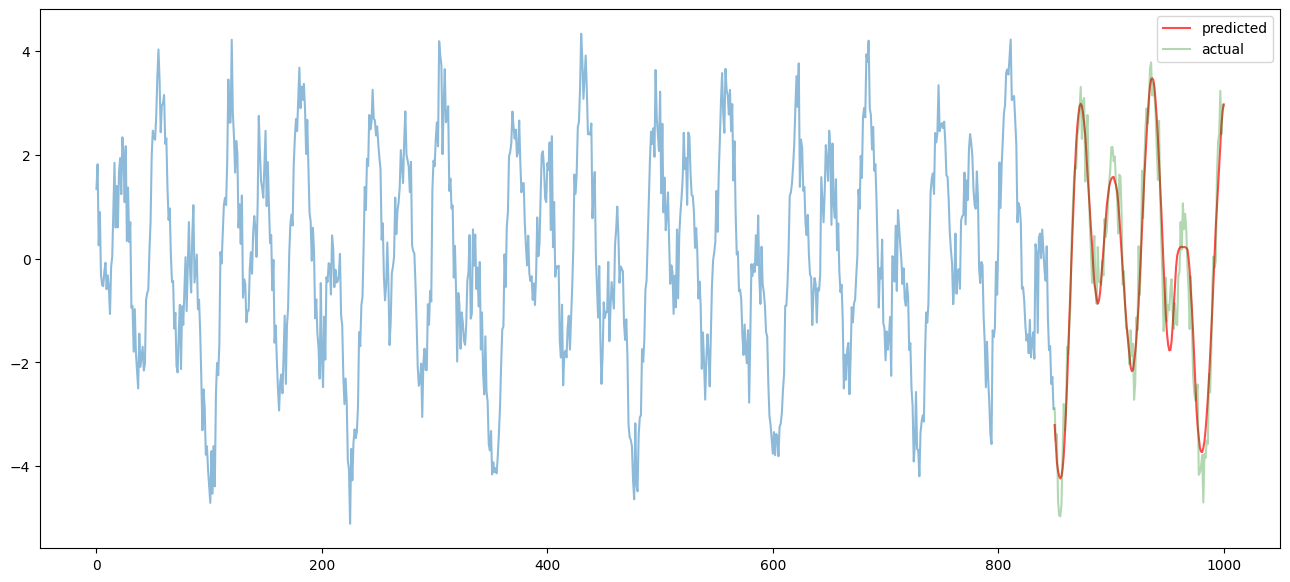
\includegraphics[width=\textwidth]{LSTM-prediction.png}
	\caption{Прогноз с использованием LSTM}
	\label{fig:fig6}
\end{figure}

\subsection{SARIMA}

ARIMA позволяет находить авторегрессионные зависимости. SARIMA (Seasonal ARIMA) учитывает так же сезонность данных. Это может быть полезным в случае с данными природного характера, как например, температура воздуха или выработка электричества.

Ряд прогнозируется довольно плохо, в случае если он имеет достаточно нетривиальную структуру. Так же, в данных может не быть явной сезонности, что ухудшает точность данного метода.

\begin{figure}[H]
	\centering
	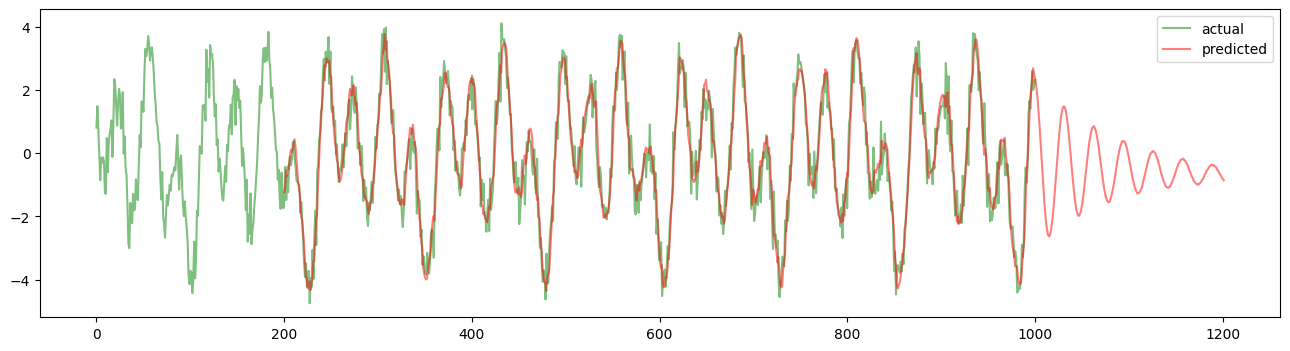
\includegraphics[width=\textwidth]{SARIMA-prediction.png}
	\caption{Прогноз с использованием SARIMA}
	\label{fig:fig2}
\end{figure}

\subsection{LSTM на матрице попарных корреляций}

\subsection{Bidirectional LSTM на матрице попарных корреляций}



\bibliography{references}
\bibliographystyle{plain}


\end{document}